\section{Introducción}

En los últimos años, la evolución en el campo de la industria ha sido tan grande que ha llegado al punto que se ha hecho necesario el desarrollo de robots para poder realizar las tareas de manera más eficaz, eficiente y segura. Estos robots pueden tener diferente apariencia y función según el ámbito al que se apliquen, desde robots industriales hasta robots para las tareas domésticas. En el campo industrial los robots pueden ser más simples ya que el entorno es principalmente estático, las tareas a desarrollar son repetitivas y automáticas, y apenas hay interacción humana. 

Pero no todos los entornos reúnen las condiciones ideales de ser estáticos y repetitivos. Por esta razón surgió la necesidad de crear robots que fueran capaces de trabajar en entornos dinámicos siendo capaces de desarrollar tareas complejas e interactuar con los seres humanos y su entorno. De esa idea de interacción humana surgieron los robots humanoides, con forma humana e inteligencia artificial, que les permite desarrollar un comportamiento y acciones más parecidas a las de los humanos. Pero para llevar a cabo esas acciones es necesario un control ya que la posibilidad de moverse trae consigo el problema de la estabilidad.

\begin{figure}[H]
\centering
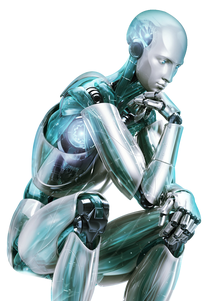
\includegraphics[scale=0.7]{imagenes/apartado_1/11_robot_humanoide}
\caption{Robot humanoide \cite{ref39}}
\label{figura1}
\end{figure}

Evitar la pérdida de equilibrio del robot durante las fases de posición estática o caminata bípeda es una tarea compleja que está relacionada con el control.

Además, pueden aparecer perturbaciones que dificulten el equilibrio. Dichas perturbaciones pueden surgir de diversas fuentes como pueden ser un empujón o un terreno irregular. El ser humano es capaz de corregirlas inconscientemente moviendo el cuerpo o cualquier articulación. Este movimiento no lo realizan los robots por sí solos por lo que para lograrlo éstos deben imitar nuestros patrones a través de la programación que se les ha proporcionado para estabilizarse por sí solos. 


\subsection{Motivaciones y origen del proyecto}

En la actualidad uno de los campos con mayor proyección en la investigación dentro del campo de la robótica es el de crear un robot capaz de desenvolverse por sí solo en el entorno de los seres humanos. De esta idea nacen los robots humanoides, robots con apariencia de ser humano que con inteligencia artificial pretenden mimetizar nuestros comportamientos para desenvolverse en entornos similares al nuestro.

La investigación ha avanzado mucho en  los últimos años debido al avance tecnológico en el que nos encontramos. 

Pero éstos tienen un problema, la estabilidad al realizar movimientos. Han surgido diversos estudios acerca de aproximarse lo máximo posible a la idea de estabilización del robot, pero dichos estudios poseen diferentes salidas debido a las interferencias de los sensores y el entorno. 

De aquí surgió la idea del actual proyecto, en el que se pretende mejorar la respuesta de los sensores, reduciendo el error, ante estímulos externos para así poder aumentar la estabilidad del robot humanoide TEO.

\subsection{Objetivos}

El actual proyecto trata sobre el estudio de los parámetros que sirven para controlar la estabilidad del robot humanoide TEO. El parámetro principal es el Zero Moment Point (ZMP), que es un indicador de estabilidad del robot \cite{ref19}. Este parámetro se obtiene a partir de la información recibida de los diferentes sensores que posee, tanto los de fuerza-par como el inercial.

Teniendo en cuenta que se van a utilizar estos sensores para medir la estabilidad, y apoyándose sobre unos modelos que están relacionados con el ZMP, los objetivos del presente trabajo son:

- Realizar un estudio del funcionamiento de los sensores, comprobar que las medidas se computan correctamente, obtener los datos y aplicarlos a los modelos.

- Verificar el modelo con los parámetros calculados a partir de la información recibida de los sensores de fuerza-par.

- Una vez que se ha verificado el modelo, desarrollar una mejora que reduzca su error.

- Aplicar dicha mejora a la IMU para que ambas medidas de ZMP coincidan.

\subsection{Marco regulador}

Debido al aumento tanto de la tecnología como de la inteligencia artificial en nuestras vidas, las grandes organizaciones gubernamentales se han visto obligadas a redactar una serie de leyes que regulen la convivencia de los robots y los humanos. Se puede considerar como precursor de las normativas a Isaac Asimov, quien estableció las tres leyes principales que todo robot debe cumplir \cite{ref1}:

\begin{enumerate}
\item ``Un robot no hará daño a un ser humano, ni permitirá con su inacción que sufra daño.''
\item ``Un robot debe obedecer las órdenes dadas por un ser humano excepto si éstas entran en conflicto con la 1ª ley.''
\item ``Un robot debe proteger su propia existencia en la medida en la que dicha protección no entre en conflicto con la 1ª y la 2ª ley.''
\end{enumerate}

Debido a la continua implantación de robots en el sector industrial y su interacción con seres humanos en un mismo espacio de trabajo, se redactaron una serie de leyes, entre las que se encuentran:

\begin{enumerate}

\item UNE-EN ISO 10218-1:2012 Robots y dispositivos robóticos. Requisitos de seguridad para robots industriales. Parte 1: Robots. (ISO 10218-1:2012) \cite{ref27}.

\item UNE-EN ISO 10218-2:2011 Robots y dispositivos robóticos. Requisitos de seguridad para robots industriales. Parte 2: Sistemas robot e integración. (ISO 10218-2:2011) \cite{ref28}.

\end{enumerate}

Estas leyes fueron concebidas para proporcionar unas pautas de seguridad en entornos en los que robot y humano comparten el mismo espacio de trabajo.

Fuera del ámbito industrial, la Unión Europea ha propuesto una serie de leyes para, en un futuro, poder regular la convivencia de robots y seres humanos en cualquier entorno \cite{ref1}:

\begin{enumerate}

\item ``Los robots deberán tener un interruptor de emergencia''

\item ``Los robots no podrán hacer daño a los seres humanos''

\item ``No podrán generarse relaciones emocionales con los robots''

\item ``Los que sean más grandes deberán tener un seguro obligatorio''

\item ``Derechos y obligaciones para los robots''

\item ``Tendrán la obligación de pagar impuestos''

\end{enumerate}

\newpage

\subsection{Planificación}

Para poder llevar a cabo el presente proyecto se ha pasado por diferentes fases, representadas en el siguiente diagrama de gantt \ref{figura2}:

\begin{figure}[H]
\centering
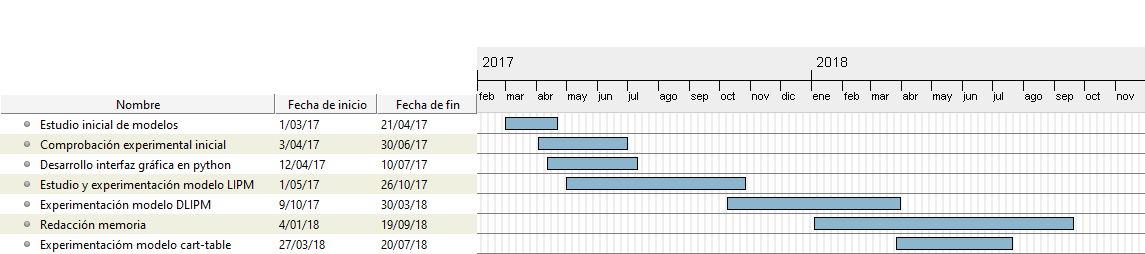
\includegraphics[width=15cm, height=4cm]{imagenes/apartado_1/12_planificacion_v1}
\caption{Planificación del proyecto}
\label{figura2}
\end{figure}

\begin{enumerate}

\item \textbf{Estudio inicial de modelos trabajados}

En esta fase inicial se realizó un estudio para una toma de contacto con los modelos empleados.

\item \textbf{Comprobación experimental inicial}

A continuación se realizaron una serie de experimentos iniciales para poder comprobar el ajuste de ambos modelos al punto de equilibrio deseado.

\item \textbf{Desarrollo de interfaz gráfica en python}

Se diseñó una interfaz gráfica en python del ZMP haciendo uso de los sensores de fuerza-par de los tobillos, detallada en el anexo \ref{aped.D}.

\item \textbf{Estudio y experimentación modelo LIPM}

Una vez que se escogió el modelo LIPM como modelo a mejorar, se realizó un estudio y una batería de experimentos para ajustar su respuesta.

\item \textbf{Experimentación modelo DLIPM}

Una vez desarrollado el nuevo modelo Dynamic LIPM, se llevaron a cabo una serie de experimentos para comprobar su validez.

\item \textbf{Estudio y experimentación modelo cart-table}

Por último, se estudió y experimentó con el modelo car-table para mejorar su respuesta ante pequeñas perturbaciones.

\end{enumerate}

\afterpage{\null\newpage}
\newpage

